\documentclass[twoside,11pt]{article}
\usepackage{jair, theapa, rawfonts}
\usepackage{times}
\usepackage{helvet}
\usepackage{courier}
\usepackage[table]{xcolor}
\usepackage{graphicx}
\usepackage{amssymb,amsmath,amsthm,amsfonts}
\usepackage[vlined,ruled,linesnumbered]{algorithm2e}

\usepackage{algpseudocode}
\usepackage{float}
\usepackage{tikz}
\usepackage{color}
\usepackage{calc}
\usepackage{subfig}

\usepackage{booktabs}
\usepackage{multirow}


\frenchspacing

\setlength{\pdfpagewidth}{8.5in}
\setlength{\pdfpageheight}{11in}

\setcounter{secnumdepth}{1}


\newcommand{\X}{\mathcal{X}}
\newcommand{\g}{\mathcal{G}}
\newcommand{\var}{\textsf{var}}
\newcommand{\Lit}{{\cal L}}

\newcommand {\SAT}{\textsf{SAT}}
\newcommand{\degr}{\textsf{d}}

\newcommand{\scc}{\textsf{scc}}
\newcommand{\FL}{\textsf{FL}}
\newcommand{\BL}{\textsf{BL}}
\newcommand{\BLap}{{\sf \widehat{BL}}}
\newcommand{\NBLap}{{\sf \overline{BL}_\downharpoonright}}
\newcommand{\BV}{\textsf{BV}}
\newcommand{\Pre}{\textsf{Pre}}

\newcommand{\tool}{{\sc Bone}\xspace}
\newcommand{\minibones}{{\sc Minibones}\xspace}
\newcommand{\NBL}{\overline{\textsf{BL}}}

\newcommand{\cls}{\textsf{cls}}
\newcommand{\cl}{\mathcal{C}}
\newcommand{\f}{\textsf{F}}
\newcommand{\Cnt}{\textsf{Cnt}}
\newcommand{\dens}{\textsf{Dnt}}

\newtheorem{theorem}{Theorem}
\newtheorem{lemma}{Lemma}
\newtheorem{corollary}{Corollary}
\newtheorem{proposition}{Proposition}
\newtheorem{definition}{Definition}
\newtheorem{example}{Example}
\newtheorem{remark}{Remark}

 \begin{document}
% The file aaai.sty is the style file for AAAI Press
% proceedings, working notes, and technical reports.
%
\title{Towards Backbone Computing: A Greedy-Whitening Based Approach}

%\author{Yueling Zhang \\ {\bf Min Zhang} \\ {\bf Geguang Pu} \\ Shanghai Key Laboratory of Trustworthy Computing \\ National Research Center of Trustworthy Embedded Software \\ East China Normal University, China  \\ {ylzhang, mzhang, ggpu} @sei.ecnu.edu.cn
%Fu Song \\ School of Information Science and Technology, ShanghaiTech University \\ songfu@shanghaitech.edu.cn}

\author{\name Yueling Zhang \email ylzhang@sei.ecnu.edu.cn \\
       \name Min Zhang \email mzhang@sei.ecnu.edu.cn \\
       \name Geguang Pu \email ggpu@sei.ecnu.edu.cn \\
       \addr  Shanghai Key Laboratory of Trustworthy Computing
        \\ National Research Center of Trustworthy Embedded Software
        \\ East China Normal University, Chin
       \AND
       \name Fu Song \email songfu@shanghaitech.edu.cn \\
       \addr School of Information Science and Technology
        \\ ShanghaiTech University, China
       \AND
       \name Jianwen Li \email jwli@sei.ecnu.edu.cn \\
       \addr }
\maketitle


\begin{abstract}
Backbone is widely used in random SAT solving, \#SAT and planning, etc.
In this paper, we propose a greedy-whitening based approach for computing backbone of propositional Boolean formulae.
We present a greedy-based algorithm with two heuristic searching strategies to compute an under-approximation of non-backbone and
a whitening-based algorithm to compute an approximation of backbone.
The exact backbone is computed by applying iterative test backbone on the approximations.
We implemented our approach in a tool \tool and conducted experiments on instances from Industrial tracks of SAT Competitions
between 2002 and 2016. For industrial benchmarks, experimental results demonstrate that \tool solves as many 34 formulae as \minibones does (72 formulae in total).
\minibones performs better on \textit{mrpp} benchmark (4\% times faster), while \tool performs better on \textit{manthey} benchmark, saving 38\% solving time.
Experiments with 6606 small formulae generated from 86 unsatisfiable formulae indicate that \tool is able to find more backbone quicker when the structure of the formulae are more complex.
\end{abstract}



\section{Introduction}
The \textit{backbone} of a satisfiable formula is a set of literals that are true in all formula's models,
which plays an important role for understanding the hardness of problems in computation complexity.
For satisfiability problem~\cite{MZKST99},  backbone provides a good explanation for the apparent inevitably high cost of heuristic search near the phase boundary.
%For instance, the presence of backbones provides a good explanation for the apparent inevitably high cost of heuristic search near the phase boundary  for satisfiability problem \cite{MZKST99}.

The identification of backbone  has many practical applications. Backbone improves the performance of the random SAT solver like  WalkSAT~\cite{SBK1993} by making biased moves in a local search~\cite{ZWR2003,MAR2007}. In addition, backbone can significantly contributes to the Lin-Kernighan local search algorithms for Travel Salesman Problem~\cite{ZWL2005}. Another recent successful application of backbones is post-silicon fault localisation in integrated circuits~\cite{ZWSM11,ZWM11}.

However, deciding whether a literal is a backbone literal is co-NP complete~\cite{Jan10}. Many heuristic approaches were proposed to compute backbone in different setting, such as model enumeration, iterative SAT-testing and filtering with modern SAT solvers.
Marques-Silva et al. conducted an experimental evaluation by integration existing algorithms with optimisations in a modern SAT solver and showed that backbone computation for large practical formulae is feasible \cite{MJML2010,JLMS12,JLM15}.


In this paper, we propose a novel Greedy-Whitening based approach \tool for computing backbones. The insight of this approach has two-folds: 1) we present a fast procedure to compute an under-approximation set of non-backbone, which prunes the search space during the computation of backbone; 2) we also computes an approximation of backbone in polynomial time, and the elements in this set have high possibility to be  backbone literals which help us to  compute the exact backbone using SAT solvers.

We implemented our approach in a tool \tool and evaluated this tool with empirical experiments. We tested 72 satisfiable industrial formulae with time limits, the formulae are selected from SAT competitions during 2002 to 2016~\footnote{http://www.satcompetition.org/}.  \tool solved 34 from satisfiable industrial formulae in 3600 seconds and reduces 21\% total solving time comparing to \minibones. Especially, for group \textit{mrpp}, \tool reduces 38\% solving time. On the other hand, we tested  6600 formulae generated automatically from 86 unsatisfiable formulae. We show that \tool is able to find more backbone quicker when the number of variables in the same clause of the formulae is in some range.

\section{Preliminaries}\label{sec:prel}

We fix a finite set  $\X$ of \emph{Boolean variables}.
A \emph{literal} $l$ is either a Boolean variable $x\in \X$ or its negation $\neg x$.
The negation of a literal $\neg x$ is $x$, i.e., $\neg\neg x=x$.
A \emph{clause} $\phi$ is a disjunction of literals $\bigvee_{i=1}^n l_i$, which may be regarded as
the set of literals $\{l_i\mid 1\leq i\leq n\}$. W.l.o.g., we assume that for every
clause $\phi$, if $l\in\phi$, then $\neg l\not\in \phi$.

A \emph{formula} $\Phi$ over $\X$ is a Boolean combination of variables $\X$.
We assume that formulae are given in conjunctive normal
form (CNF), namely each formula $\Phi$ is a conjunction of clauses $\bigwedge_{i=1}^n\phi_i$ which may be regarded as a set of clauses $\{\phi_i\mid 1\leq i\leq n\}$. Given a formula $\Phi$, let $\var(\Phi)$ (resp. $\Lit(\Phi)$  and $\cls(\Phi)$) denote the set of variables (resp. literals and clauses) used in $\Phi$.
We use $\|\Phi\|$ to denote $\sum_{\phi\in\Phi}|\phi|$.
We use $\neg\Lit(\Phi)$ to denote the set $\{\neg l \mid l\in \Lit(\Phi)\}$.
The \emph{size} $|\Phi|$ of $\Phi$ is the number of literals of $\Phi$.
Given a formula $\Phi$ and a literal $l\in\Lit(\Phi)$,
let $\Phi_{l}\subseteq \Phi$ be the set of clauses $\{\phi\in\Phi\mid l\in\phi\}$.
%and $\Phi_\downarrow$ be the set $\{(l,\Phi_{\downarrow l})\mid l\in \Lit(\Phi)\}$.
%Given a clause $\phi$ of $\Phi$, let $\sharp(\phi,\Phi)$ be the count of occurrence of $\phi$ in the second components of tuples in $\Phi_\downarrow$.
%Given a set of clauses $\Phi_{l_x}$, let $\Phi_{l_x}^0 = \Phi_{\downarrow l}$, let $\Phi_{\downarrow l}^k$, $\Phi_{\downarrow l}^{k-1}\subseteq\Phi_{\downarrow l}^k\subseteq\Phi_{\downarrow 1}^{k+1}\subseteq\Phi (k \geq 1)$ be the set of clauses $\{\phi\in\Phi \mid \exists l\in\Lit(\Phi_{\downarrow l}^{k-1}), \neg l\in\Lit(\phi)\} (k \geq 1)$.

%A \emph{partial assignment} is a partial function $\lambda:\X\rightarrow \{0,1\}$ which assigns to each defined variable a Boolean value. Let $\lambda_x$ denote the partial assignment such that for every $y\in \X$, $\lambda_x(y)=\lambda(x)$ if $x=y$, otherwise $\lambda_x(y)$ is undefined.
%A \emph{complete assignment} is a partial assignment in which all the variables are defined.

An \emph{assignment} is a function $\lambda: \X \rightarrow \{0,1\}$, where $1$ (resp. $0$) denotes true (resp. false).
Given an assignment $\lambda$ and a literal $l$ that is $x$ or $\neg x$, let $\lambda[\neg l]$ be the assignment which is equal to $\lambda$
except for $\lambda[\neg l](x)=\neg \lambda(x)$. Given a set of variables $x=\{x_1,...,x_n\}$, let $\lambda[\neg L]$ denote the assignment
$\lambda[\neg x_1]...[\neg x_n]$.
An assignment $\lambda$ \emph{satisfies} a formula $\Phi$, denoted by $\lambda\models \Phi$, iff assigning $\lambda(x)$ to $x$ for $x\in\var(\Phi)$ makes $\Phi$ true.

\iffalse
An assignment $\lambda$ is a \emph{model} of $\Phi$ if $\lambda\models \Phi$.
Given two models $\lambda_1$ and $\lambda_2$ of $\Phi$, $\lambda_2$ can be \emph{generated} from $\lambda_1$, denoted by $\lambda_1\Rightarrow_\Phi\lambda_2$, if there exists a literal $l$ such that $\lambda_2=\lambda_1[\neg l]$.
Let $\Rightarrow^*_\Phi$ denote the \emph{reflexive transitive} closure of $\Rightarrow_\Phi$.
Formally, for every model $\lambda$ of $\Phi$, $\lambda\Rightarrow^*_\Phi\lambda$ and $\lambda_1\Rightarrow^*_\Phi\lambda_3$ if $\lambda_1\Rightarrow^*_\Phi\lambda_2$ and $\lambda_2\Rightarrow^*_\Phi\lambda_3$.
A \emph{model cluster} $\cl_\Phi(\lambda)$ of $\lambda$ is the set of models $\{\lambda'\mid \lambda\Rightarrow^*_\Phi\lambda'\}$.
A literal $l$ is a \emph{frozen literal} in a model $\lambda$ of $\Phi$,
if $l$ takes the same value in all the models of $\cl_\Phi(\lambda)$. Let $\FL(\Phi,\lambda)$ denote the set of all the frozen literals
in the model $\lambda$ of $\Phi$. %, and $\FL(\Phi)$ denote the intersection of $\FL(\Phi,\lambda)$ for all the models $\lambda$ of $\Phi$.
\fi

A formula $\Phi$ is \emph{satisfiable} iff there exists an assignment $\lambda$ such that $\lambda\models \Phi$.
Given a formula $\Phi$, the \emph{satisfiability problem} is to decide whether $\Phi$ is satisfiable or not.

\smallskip

\begin{definition}[Backbone]
\label{def:backbone}
Given a satisfiable formula $\Phi$, a literal $l$ is a \emph{backbone literal} of $\Phi$ iff for all assignments $\lambda$ such that $\lambda\models\Phi$,
$\lambda\models l$. The \emph{backbone} $\BL(\Phi)$ of $\Phi$ is the set of backbone literals of $\Phi$.
\end{definition}

\iffalse
Since a backbone literal takes same value in all the models and a frozen literal takes same value in a model cluster instead of all the models,
we get that:

\begin{proposition}\label{prop:Frozen-backbone}
For any formula $\Phi$ and model $\lambda$ of $\Phi$, $\BL(\Phi)\subseteq\FL(\Phi,\lambda)$.
\end{proposition}
Computing $\FL(\Phi,\lambda)$ of a given model is in polynomial time. However, the generation of the first model in each $\cl_\Phi(\lambda)$ still needs a SAT testing.
\fi

It is known that the backbone $\BL(\Phi)$ for each formula $\Phi$ is unique \cite{JLM15}.
The backbone of an unsatisfiable formula can be defined as an empty set. Therefore, in this work, we focus on satisfiable formulae.
We will use $\NBL(\Phi)$ to denote the set
$\Lit(\Phi)\setminus \BL(\Phi)$.

\begin{theorem}
\label{thm:co-NP}\cite{Jan10}
Given a satisfiable formula $\Phi$ and a literal $l$, deciding whether $l$ is a backbone literal is co-NP-complete.
\end{theorem}

\begin{definition}[Satisfied literal]
Given a model $\lambda$ of the formula $\Phi$ and a clause $\phi\in\Phi$, for each literal $l\in\phi$, $l$ is a \emph{satisfied literal}
of $\phi$ iff $\lambda\models l$. $l$ is a \emph{unique satisfied literal} of $\phi$ if there is no satisfied literal $l'$ of $\phi\setminus\{l\}$.
\end{definition}

Let us consider the formula $\Phi=\{\neg x_1 \vee \neg x_2, x_1, x_3 \vee x_4\}$,
$\var(\Phi)=\{x_1, x_2, x_3, x_4\}$, $\Lit(\Phi)=\{\neg x_1, x_1, \neg x_2, x_3, x_4\}$, $\Phi_{\neg x_2}=\{\neg x_1 \vee \neg x_2\}$ and $\BL(\Phi)=\{x_1, \neg x_2\}$.
Given a model $\lambda$ such that $\lambda(\neg x_1)=1,\lambda(\neg x_2)=0$. The satisfied literal of clause ($\neg x_1\vee\neg x_2$) is $\neg x_1$.

Given a formula $\Phi$ and a literal $l$, let $\Cnt(\Phi,l)$ denote the number of occurrence of $l$ in $\Phi$.
The \emph{density} $\dens(\Phi,l)$ of $l$ in $\Phi$ is defined as
\[
\dens(\Phi, l)=\frac{\Cnt(\Phi,l)}{\|\Phi_l\|}.
\]

\section{Overview of our Approach}\label{sec:overview}
In this section, we present the overview of our approach, called BONE, for computing backbone. Figure 1 depicts the framework of BONE.
% We show the overview of our approach \tool in Figure \ref{flow}.
Taking a satisfiable formula $\Phi$ as an input, \tool first computes a subset of non-backbone $\NBLap(\Phi)\subseteq \NBL(\Phi)$.
Then, \tool computes
% an intermediate set of backbone $\BLap(\Phi)$
approximation $\BLap(\Phi)$ of the backbone
based on the set $\NBLap(\Phi)$, where each literal $l\in \BLap(\Phi)$ has a high possibility to be a backbone literal of $\Phi$.
Finally, \tool removes non-backbone literals from $\BLap(\Phi)$ and adds backbone literals into $\BLap(\Phi)$ to compute the exact backbone of $\Phi$.
\begin{figure*}[t]
   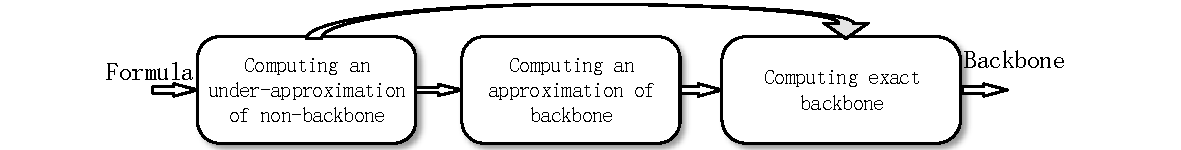
\includegraphics[scale=0.75]{Framework}
  \hspace*{30mm} 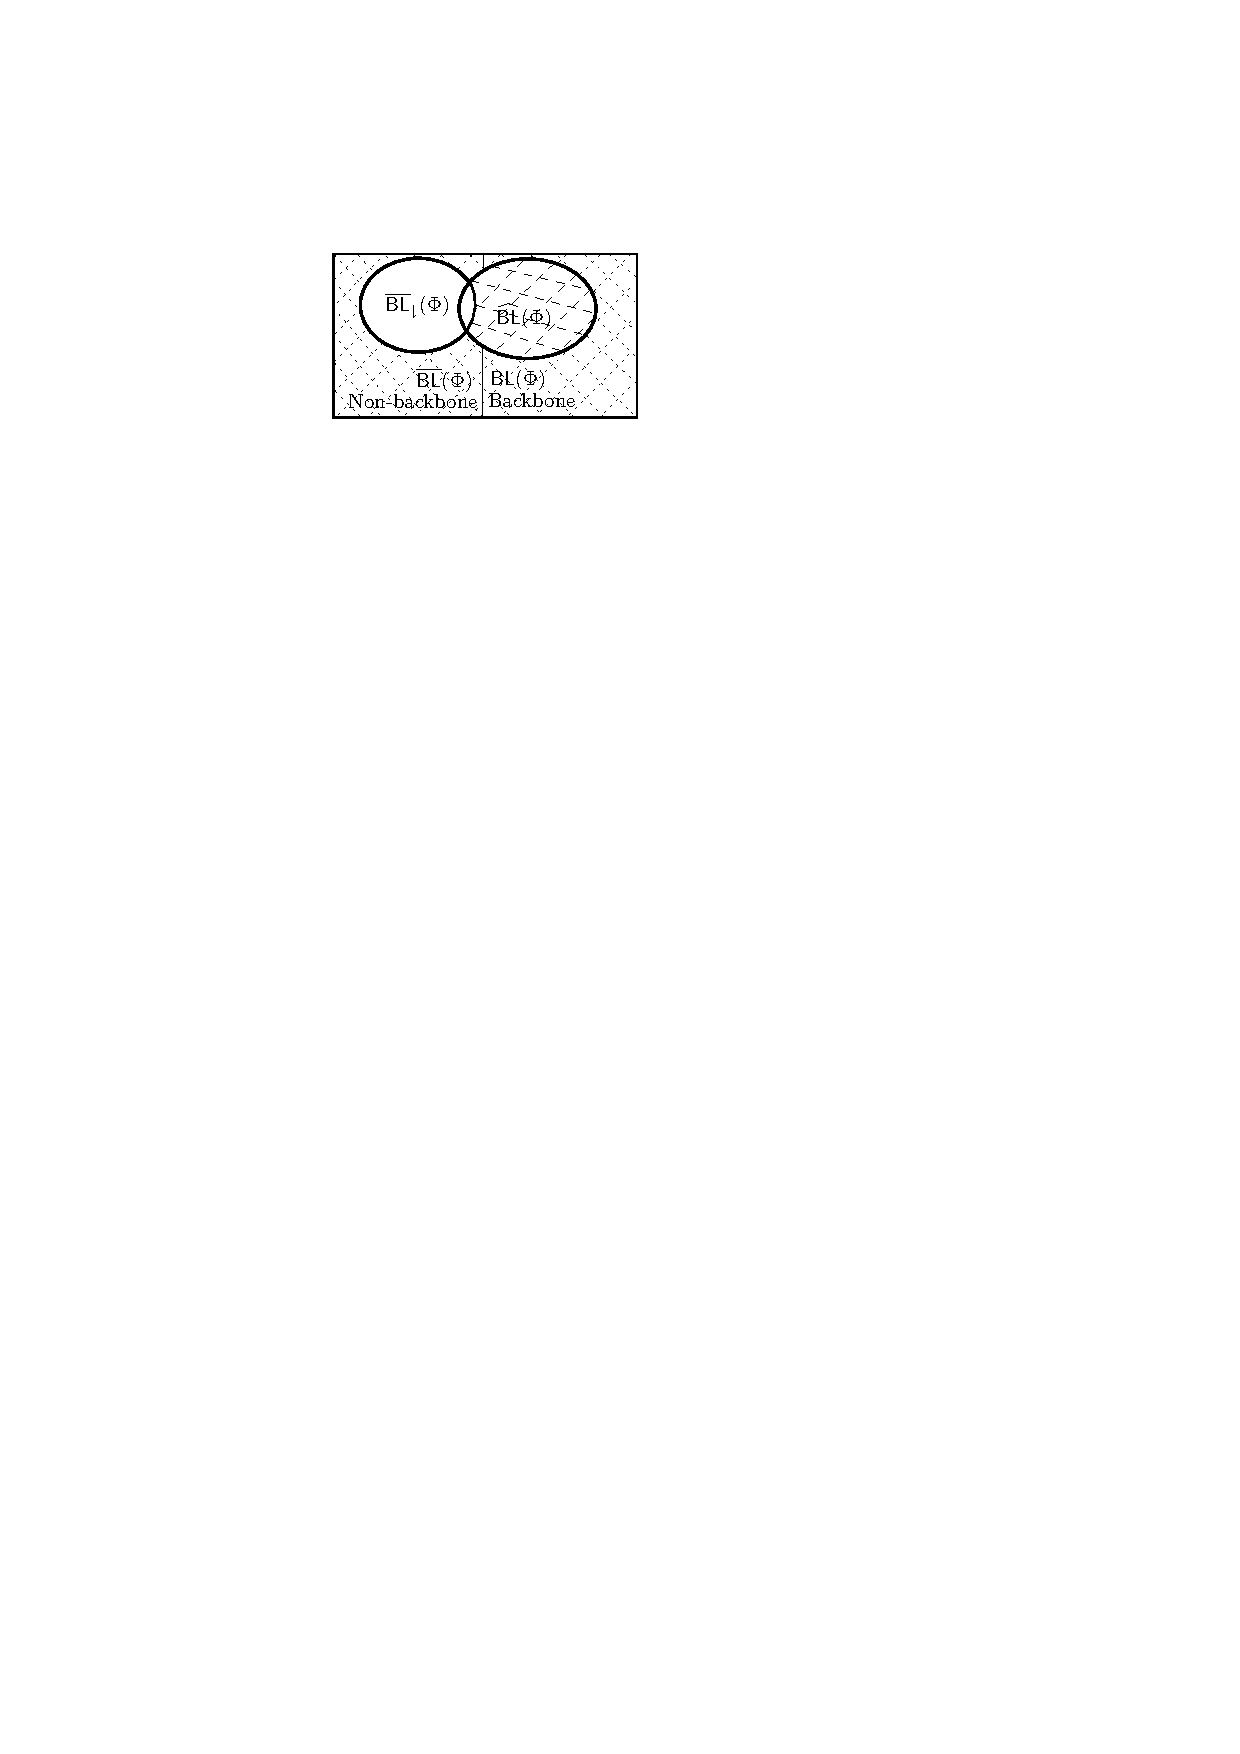
\includegraphics[scale=0.75]{Fig-backbone}
   \caption{Overview of our approach}
   \label{flow}
\end{figure*}

% As shown in Figure \ref{flow}, $\NBLap(\Phi)$ only contains a part of non-backbone literals.
% Most of the literals in $\BLap(\Phi)$ are backbone, only a small part of them is non-backbone.
% With more known backbone literals, SAT testings are accelerated.

\medskip
\noindent{\bf Computing an under-approximation of non-backbone.}
Given a satisfiable formula $\Phi$, we first compute a model $\lambda$ of $\Phi$ by calling a SAT solver.
From the model $\lambda$, we compute a base under-approximation of non-backbone.
Later, we apply a Greedy-based algorithm to add more non-backbone literals into the base set, which results in $\NBLap(\Phi)$.

%The algorithm iteratively computes new models based on the original model $\lambda$, by changing exactly one literal at each iteration. K models will be generated after the k iterations. New non-backbone literals are found from each new model. The main idea of Greedy-based algorithm is changing the literal that satisfies the least clauses at each iteration.
% Choosing the literal that satisfies the least clauses will affects the least clauses, which lead to a higher possibility of finding a new model.
The algorithm iteratively computes new models until no new model can be found. We choose to change the literal that satisfies the least clauses at each iteration, as the number of clauses effected by this literal is the least one, provided a higher possibility to find a new model. K models will be generated after the k iterations. New non-backbone literals are found from each new model.

\medskip
\noindent{\bf Computing an approximation of backbone.}
At this step, we apply a Whitening-based algorithm to compute an approximation $\BLap(\Phi)$.
Whitening Algorithm was used to compute \emph{essential nodes} that cannot be colored as white without changing the color of its adjacent nodes in a graph coloring problem.


We consider essential nodes as 'possible' backbone literals in backbone computing.
To increase the proportion of backbone literals found by Whitening Algorithm, we use two heuristic strategies to refine Whitening Algorithm.
First, we check whether the generated assignment is a model to eliminate some of the non-backbone literals returned by Whitening-based Algorithm.
Moreover, we use assumptions features of MINISAT \cite{JLM15} to find some accurate backbone literals.
With the refinement of heuristic strategies, Whitening-based Algorithm is able to return a set of literals that are highly likely to be backbone.


\medskip
\noindent{\bf Computing exact backbone.}
Based on $\BLap(\Phi)$, we use Algorithm 3 (Iterative Algorithm) from \cite{JLM15} to compute backbone.
This algorithm uses SAT solvers to test whether a literal is a backbone literal or not.
For instance, if $\Phi\wedge \neg l$ is unsatisfiable but $\Phi$ is satisfiable, then $l$ must be a backbone literal of $\Phi$.

We first iteratively select one literal $l$ from $\BLap(\Phi)\setminus \NBLap(\Phi)$ such that $\lambda \models \neg l$ and test $l$ by checking the satisfiability of $\Phi\wedge l$ (dashed area in Figure \ref{flow}).
If $l$ is a backbone, we will add $l$ into $\Phi$ as a clause. Adding known backbone literals into $\Phi$ as clauses potentially speedups the later SAT testing \cite{JLM15,MPA2015}.
Then, we do the same testing for literals from $\Lit(\Phi)\setminus (\NBLap(\Phi)\cup\BLap(\Phi))$ (dotted area in Figure \ref{flow}).
After this step, the exact backbone and non-backbone are found.


Comparing to the approach of directly test all literals in $\Lit(\Phi)$, there are two contributions of \tool.
One is that we reduce the number of SAT calls using the known non-backbone literals $\BLap(\Phi)$.
The another one is that we first check literals that have high probability to be backbone literals so that backbone literals can be found as early as possible.





\section{Greedy-based Computing $\NBLap(\Phi)$} \label{sec:greedy}
In this section, we propose an algorithm to compute the under approximation of non-backbone, namely Greedy-based Algorithm. As mentioned in Section \ref{sec:overview}, Greedy-based Algorithm is a straight forward algorithm which is able to compute parts of non-backbone in $O(n^2)$ time. It's able to reduce the number of total SAT calls since literals in $\NBLap(\Phi)$ don't need SAT testings. Experiments show that Greedy-based Algorithm reduces 5\% solving time.

\subsection{Computing $\NBLap(\Phi)$ Using one model}

Given a formula $\Phi$, we first compute a model $\lambda$ using SAT solver. We then compute the set of non-backbone literals using $\lambda$, referred as $L(\Phi,\lambda)$.
% Every literal in $L(\Phi,\lambda)$ only satisfies clauses that has at least two satisfied literals, i.e., $\forall l\in L(\Phi,\lambda), \forall \phi\in\Phi_l, \exists l'\in\phi, \lambda(l')=1$.
To compute $L(\Phi,\lambda)$, we first find clauses that have at least two satisfied literals and put them into a set, refereed as $\Phi_{\models_2}$. We then scan all literals in $\Lit(\Phi)$, and skip literal $l$ and $\neg l$ if $l$ satisfies a clause $\phi\notin\Phi_{\models_2}$. Otherwise, then we put it into $L(\Phi,\lambda)$.

\begin{algorithm2e}
\SetKwInOut{Input}{Input}
\SetKwInOut{Output}{Output}
\SetAlgoShortEnd
\SetFillComment
\Input{a satisfiable formula $\Phi$ and a model $\lambda$ of $\Phi$}
\Output{a set of literals $\NBLap(\Phi)$}
$\NBLap(\Phi):=L(\Phi,\lambda)$\;
\Return $\NBLap(\Phi)$\;
\caption{Na\"{\i}ve Algorithm: Computing non-backbone literals using $\lambda$}
\label{alg:greedy}
\end{algorithm2e}

The only line in this na\"{\i}ve Algorithm is computing the non-backbone literals set of a given model $\lambda$.

\begin{theorem} \label{lem:navie}
 $L(\Phi,\lambda)\subseteq\NBL(\Phi)$.
\end{theorem}

\begin{proof}
Suppose a literal $l\in\L(\Phi,\lambda)$. According to the Na\"{\i}ve Algorithm, $\lambda(l)=1$, and there must exists a literal $l'$ in any clause $\phi$ that contains $l$, such that $l'\neq l\wedge\lambda(l')=1$. Therefore, there must exist a model $\lambda'=\lambda[\neg l]$. It concludes that $l$ is a non-backbone literal of $\Phi$, i.e., $l\in\NBL(\Phi)$.
\end{proof}

\medskip

\subsection{Computing $\NBLap(\Phi)$ Using Greedy-based Algorithm}

To save more SAT testings, we propose the Greedy-based algorithm shown in Algorithm \ref{alg:greedy} to get more non-backbone literals. We use $HS$ to denote the heuristic strategy of greedy algorithm. 
% $HS$ greedily find the literal that satisfied the least clauses.
$C$ is an order set of literals, resulted from the heuristic strategy $HS$.
When changing the assignment of a literal $l$, the less clauses $l$ satisfies, the less clauses are affected, the higher possibility that a new model is found.

\begin{algorithm2e}
\SetKwInOut{Input}{Input}
\SetKwInOut{Output}{Output}
\SetAlgoShortEnd
\SetFillComment
\Input{a satisfiable formula $\Phi$ and a model $\lambda$ of $\Phi$}
\Output{a set of literals $\NBLap(\Phi)$}
$\NBLap(\Phi):=L(\Phi,\lambda)$\; \label{alg1:init}
$C:={\sf HS}(\Phi)$\; \label{alg1:c}
$i:=0$\;
\While{$i<|C|$}{ \label{alg1:loop}
    $i:=i+1$,  $l:=C[i]$\;
    \If{$\lambda[\neg l]\models \Phi$}{ \label{alg1:sat_test}
        $\NBLap(\Phi):=\NBLap(\Phi)\cup L(\Phi,\lambda[\neg l])$\; \label{alg1:coml}
        $\lambda:=\lambda[\neg l]$\;
    }
}
\Return $\NBLap(\Phi)$\;
\caption{Greedy-based algorithm}
\label{alg:greedy}
\end{algorithm2e}
Given a formula $\Phi$ and a model $\lambda$, we construct the ordered set of literals $C$ according to $HS$ at Line \ref{alg1:c}. From Line \ref{alg1:loop}, we start to change the assignment of the literal in $C$ one by one. At Line \ref{alg1:sat_test}, for each selected literal $l$, we construct a new assignment $\lambda[\neg l]$ from the model
$\lambda$ and check whether  $\lambda[\neg l]$ satisfies $\Phi$ in polynomial time. If $\lambda[\neg l]$ satisfies $\Phi$, then we add the set of non-backbone literals $L(\Phi,\lambda[\neg l])$ into $\NBLap(\Phi)$, and
assign $\lambda[\neg l]$ to $\lambda$ which will be severed as the model of $\Phi$ at the next step.

\begin{theorem}
$\NBLap(\Phi)\subseteq\NBL(\Phi)$.
\end{theorem}

\begin{proof}
Suppose a literal $l\in\NBLap(\Phi)$, if $l\in L(\Phi,\lambda)$, $l\in\NBL(\Phi)$ (Theorem \ref{lem:navie}). Otherwise, we know that there must exists a model $\lambda'$, $l\in L(\Phi,\lambda')$ according to Line \ref{alg1:sat_test}. Since $L(\Phi,\lambda')\subseteq\NBL(\Phi)$ (Theorem \ref{lem:navie}), $l\in\NBL(\Phi)$. It concludes that $\NBLap(\Phi)\subseteq\NBL(\Phi)$.
\end{proof}

\begin{theorem}
The complexity of Greedy-based Algorithm is $O(n^2)$.
\end{theorem}

\begin{proof}
Started from Line \ref{alg1:init}, we scan all clauses to count number of satisfied literals, and scan all variables to compute $L(\Phi,\lambda)$. The complexity of Line \ref{alg1:init} is $O(n^2)$. With the information collected from Line \ref{alg1:init}, Line \ref{alg1:c} will be finished in $O(nlogn)$ time since it needs to sort a set of literals decreasingly according to $HS$.  Line \ref{alg1:loop} scan all literals, the complexity is $O(n)$. With the information from Line \ref{alg1:init}, Line \ref{alg1:sat_test} will be finished in $O(1)$ time. The complexity of the loop started from \ref{alg1:loop} is $O(n)$. The total complexity of Greedy-based Algorithm is $O(n^2)$.
\end{proof}

Greedy-based Algorithm saved 5\% solving time in total. With non-backbone literals recognized ahead, SAT testing numbers are reduced. Backbone computing is expediting by the save of SAT testings.

After computing non-backbone under-approximation $\NBLap(\Phi)$, we construct a set of literals as MINISAT assumptions, which contains literals that are not in $\NBLap(\Phi)$. The interface of assumption in MINISAT is able to return the reason why the given formula is not satisfied under the given assignment (assumption). For example, given a formula $\Phi:=a\wedge(b\vee c)\wedge(a\vee\neg b\vee \neg c)$, $\Phi$ is satisfiable. Given an assumptions $\gamma:=\neg a\wedge\neg b\wedge \neg c$, there does not exist a model of $\Phi$ that satisfy $\Phi$ and $\gamma$ at the same time, $\Phi$ is not satisfied under the assumption $\gamma$, and the reason is $\neg a$. In this case, given an assumption $\gamma$, there is exactly one unsatisfiable under assumption reason of a satisfiable formula $\Phi$, then $a$ must be the backbone of $\Phi$. If there are more than 2 unsatisfiable reasons, there is a chance that none of the reasons is backbone literal. For instance, if $a$ and $b$ are reasons of a given formula with assumptions, it can only indicate that it doesn't exist a model that both $a$ and $b$ are assigned to TRUE, but it's possible that there exists models where $a$ is assigned to TRUE and $b$ is assigned to FALSE, and vice visa. 

We construct an assumption $\gamma:=\Lit(\Phi)\setminus\NBLap(\Phi)$ and find more backbone by testing satisfiability under assumption of $\gamma$. Compared with \cite{JLM15}, less literals are tested, it will reduce the number of total SAT testing. Since a part of non-backbone are removed ahead from assumption, it eliminate some of the reasons where none literals in it is backbone. In this way, removing non-backbone increases the performance of backbone finding using assumptions.   

 
\section{Whitening-based Computing $\BLap(\Phi)$}
In this section, we use $\NBLap(\Phi)$ to compute more non-backbone literals and approximation $\BLap(\Phi)$ of backbone. We fix the satisfiable formula $\Phi$. $\BLap(\Phi)$ is a set of literals with high possibility to be backbone. ll approaches to test backbone requires a SAT testing. Suppose we just use pure iterative SAT testing \cite{JLM15} for the rest of $k$ unknowing variables without computing $\BLap(\Phi)$. Once a backbone is found from testing, it will prune the searching space in the solving of the formula. Rest of testing benefit from this. If a non-backbone is found, no searching spaces will be pruned, no benefit is provided. Therefore, the earlier we test a backbone literal, the more benefits provided from the literal.

Backbone are the essential variables of a formula. In SAT solving, conflicts will always arise at the end of a search if the assignment of a backbone literal is not suitable. Same situation happened in graph coloring problem, a graph can't be k-colored if the essential nodes are not colored properly.

\cite{Par03} proposed an Whitening algorithm which was supposed to determine nodes that always have the same color in all legal colorings of the coloring problem. Since computing backbone is a co-NP problem and graph coloring is a NP problem, we are able to apply Whitening Algorithm in backbone computing.
However, Whitening Algorithm was designed to prove those non-white nodes are essential in coloring. Therefore, the result variables are not always non-backbone.
Algorithm \ref{alg:white} shows Whitening Algorithm in backbone computing. It tries to rule out non-essential variables (non-backbone).

Given a satisfiable formula $\Phi$ and a model $\lambda$ of $\Phi$,
Algorithm \ref{alg:white} computes non-essential literals by generating new models from $\lambda$ without a SAT test.
Algorithm \ref{alg:white} first computes a set of clauses $W_c$ that have at least two satisfied literals and a set of literals $W_l$ that only satisfy $W_c$, i.e., $\forall l\in W_l, \lambda(l)=1\wedge \Phi_l\subseteq W_c$. Institutively, $W_l$ equals to $L(\Phi,\lambda)$ at this step.

Started from Line \ref{alg2:loop}, Algorithm \ref{alg:white} iteratively extend $W_c$ and $W_v$. A clause is added to $W_v$ if it contains at least one literal $l$ that $\neg l\in W_l$. $W_v$ is extended accordingly. Suppose a clause $\phi\notin W_c$ contains $l_1$, such that $\neg l_1\in W_l$. Since for all clauses that contains $\neg l_2$, there exists another literal that also satisfies that clause, therefore, $\lambda[\neg l_1]$ is another model of $\Phi$. $\phi$ will be added to $W_c$ at Line \ref{alg2:inital} if the given model is $\lambda[\neg l_1]$.

\begin{algorithm}
\SetKwInOut{Input}{Input}
\SetKwInOut{Output}{Output}
\SetAlgoShortEnd
\SetFillComment
\Input{a formula $\Phi$ and a model $\lambda$ of $\Phi$}
\Output{white clauses $W_c$ and white variables $W_v$}
$W_c:= \{\phi\in\Phi \mid \exists l_1,l_2\in\phi: \ \lambda\models l_1\wedge l_2\}$\; \label{alg2:inital}
$W_v:=\{x\in \var(\Phi)\mid \lambda\models x\wedge x\not\in \Lit(\Psi\setminus W_c),
        \ \lambda\models \neg x\wedge \neg x\not\in \Lit(\Psi\setminus W_c)\}$\;
\Repeat{No Update of $W_c$ and $W_v$}{ \label{alg2:loop}
   $W_c := W_c \cup \{\phi\in\Phi \mid \var(\phi)\cap W_v\neq \emptyset \}$\; \label{alg2:wc}
   $W_v := W_v \cup \{x\in \var(\Phi)\mid \lambda\models x\wedge x\not\in \Lit(\Psi\setminus W_c),
        \ \lambda\models \neg x\wedge \neg x\not\in \Lit(\Psi\setminus W_c)\}$
}
\Return $(W_c, W_v)$\;
\caption{Whitening algorithm}
\label{alg:white}
\end{algorithm}

However, the result of Algorithm \ref{alg:white} may contains backbone literal. Actually, the result of Algorithm \ref{alg:white} may both contains backbone and non-backbone, also, it may fail to find some of the backbone and non-backbone.

Example:
Consider a formula
\[(\neg a\vee b\vee\neg c)\wedge(\neg a\vee\neg b\vee c)\wedge(\neg a\vee b\vee d)\wedge(\neg c\vee d)\wedge(a\vee d)\]
The result of Whitening algorithm is all variables are whiten. Actually, variable $d$ is a backbone variable. There doesn't exist a model $\lambda$ such that $\lambda(\neg d)=1$. Therefore, it's not correct to directly apply Algorithm \ref{alg:white} to backbone computing.

The reason of inaccuracy of Algorithm \ref{alg:white} is as follows: at Line \ref{alg2:wc}, no clause is removed from $W_c$ in order to guarantee the termination of Algorithm \ref{alg:white}; during the change of assignment, some of the clauses doesn't has at least two satisfied literals any more, it affect the non-backbone selection.

To fix this problem, we record the current assignment at each iteration and check the satisfiability of it in polynomial time. The algorithms are shown in Algorithm \ref{alg:ewhite}. At Line \ref{alg3:loopstart}, we start to extend $W_l$ and $W_c$.
We iteratively change the assignment of $l_i\in W_l$, generating a group of models $\lambda[\neg l_i]$, and try to find another non-backbone $l'$ with $\lambda[\neg l_i]$.
We use \Pre(l) to record the literals that has changed assignments before adding $l'$ to $W_l$.
For every literal $l$ in $W_l$, the clauses $\phi\in\Phi_{\neg l}$ that contains $\neg l$ are added to $W_c$. Given a model $\lambda[\neg l]$, all clauses that contains $\neg l (i.e. \Phi_{\neg l})$ have at least two satisfied literals, one is $\neg l$, the other is one of the satisfied literals of model $\lambda$ (because the only difference between $\lambda$ and $\lambda[\neg l]$ is the assignment of $l$, the other assignments remains the same).
Meanwhile, $W_l$ will be extended since there are more generated models. Algorithm \ref{alg:ewhite} will eventually terminate because both $W_l$ and $W_c$ keep increasing, they will stop extension and remain the same after several generations.
At Line \ref{alg3:test}, we test whether the current assignment generated from \Pre(l) is a model. The test will be finished in P-time, without calling a SAT solver. The assignment $\lambda[\neg (\Pre(l)\cup \{l\})]$ may not be a model because $W_c$ does not shrink together with the change of the assignments. For instance, if a clause only has two satisfied literals $l_1,l_2$, after two iterations started from Line \ref{alg3:loopstart}, both $l_1$ and $l_2$ are assigned to 0, the assignments of the rest literals remain the same, then $\lambda[\neg l_1,\neg l_2]$ is no longer a model of the given formula.

\begin{algorithm}
\SetKwInOut{Input}{Input}
\SetKwInOut{Output}{Output}
\SetAlgoShortEnd
\SetFillComment
\Input{a satisfiable formula $\Phi$ and a model $\lambda$ of $\Phi$}
\Output{a set of literals $\NBLap(\Phi)$}
$W_c:=\{\phi\in\Phi\mid \exists l_1,l_2\in\phi: \lambda\models l_1\wedge l_2\}$\;\label{alg3:l1}
$W_l:=\{\lambda(l)=1\mid \forall\phi\in\Phi_l: \phi\in W_c\}$\; \label{alg3:l2}
$\forall l\in W_l, \Pre(l)=\emptyset$\;
\Repeat{No update of $W_l$}{ \label{alg3:loopstart}
    \For{$l\in W_l$}{
        \For{$\phi\in\Phi_{\neg l}$}{
            $W_c:=W_c\cup\phi$\;
        }
        \For{$l'\notin W_l\wedge l'\in\Phi_{\neg l}$}{
            \If{$\forall\phi'\in\Phi_{l'}: \phi'\in W_c$}{
                \If{$\lambda[\neg (\Pre(l)\cup \{l\})]\models\Phi$}{ \label{alg3:test}
                    $W_l:=W_l\cup l'$\;
                    $\Pre(l'):=\Pre(l)\cup l$\;
                }
            }
        }
    }
}\label{alg3:loopend}
$\NBLap:=W_l$\;
\Return $\NBLap(\Phi)$\;
\caption{Whitening-based algorithm}
\label{alg:ewhite}
\end{algorithm}



However, the set $F(\Phi,\lambda)$ also contains non-backbone literals. We propose another heuristic strategy to remove non-backbone literals from $F(\Phi,\lambda)$.

Our strategy is based on the observation of the relationship between $W_c(\Phi,\lambda)$ and backbone literals.
Consider the formula $\Phi=(a\vee\neg b)\wedge(b\vee\neg c)\wedge(c\vee\neg a)$ and the model $\lambda$ such that $\lambda(a)=\lambda(b)=\lambda(c)=1$. The backbone of the formula $\Phi$ is $\emptyset$, because the assignment $\lambda'$ such that $\lambda'(a)=\lambda'(b)=\lambda'(c)=0$ is also a model of $\Phi$.
However, by Algorithm \ref{alg:whitening},
$W_v(\Phi,\lambda)=\emptyset$, from which we get that $F(\Phi,\lambda)=\Lit(\Phi)$. To remove the non-backbone literals $a, \ b, \ c, \ \neg a, \ \neg b$ and  $\neg c$
from $F(\Phi,\lambda)$,  we introduce a dependency graph to characterize such literals $a, \ b, \ c, \ \neg a, \ \neg b$ and  $\neg c$ from  the given formula $\Phi$.


Given a formula $\Phi$, the \emph{dependency graph} $G_\Phi$ of $\Phi$ is a directed graph $(V,E)$, where
$V=\Lit(\Phi)$ is a finite set of vertices, and $E\subseteq V\times \Phi\times V$ is a finite set of labeled edges such that
$(l_1,\phi, l_2)\in E$ iff $l_1,\neg l_2\in \phi$.

Figure \ref{fig:depend} depicts the dependency graph of the formula $\Phi=\phi_1\wedge\phi_2\wedge\phi_2$, where
$\phi_1=(a\vee\neg b)$, $\phi_2=(b\vee\neg c)$ and $\phi_3=(c\vee\neg a)$.
 \begin{figure}
    \centering
    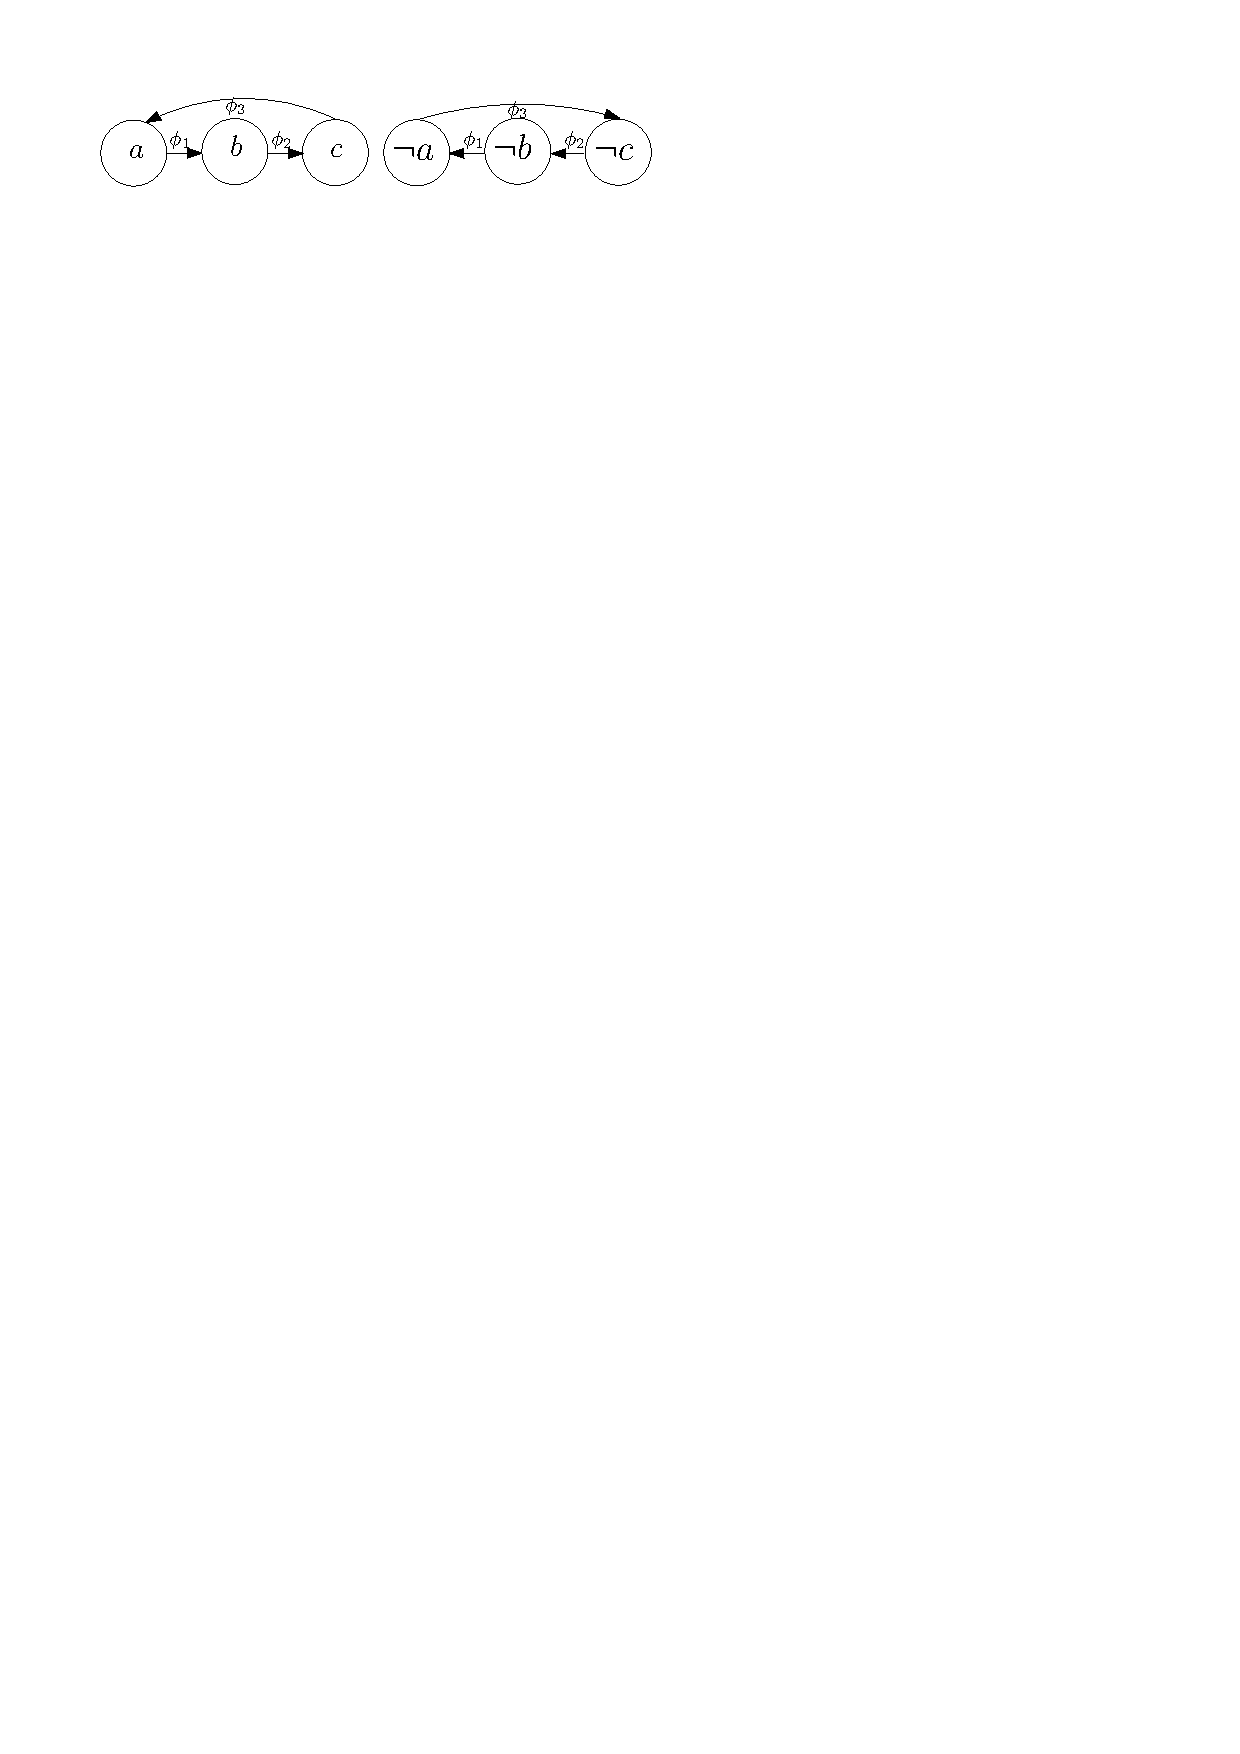
\includegraphics[scale=0.7]{dependency.pdf}
   \caption{Dependency graph of $(a\vee\neg b)\wedge(b\vee\neg c)\wedge(c\vee\neg a)$}
   \label{fig:depend}
\end{figure}

A \emph{path} $\pi$ of a dependency graph $G_\Phi=(V,E)$ is a sequence $l_1...l_n$ of nodes such that for every $i:\ 1\leq i<n$, $(l_i,\phi_i,l_{i+1})\in E$.

A \emph{simple cycle} $c$ of $G_\Phi$ is a path of $G_\Phi$ such that the starting and ending nodes are identical and no repetitions of other nodes.
We use $G_\Phi^{c}$ to denote the set of all the simple cycles of $G_\Phi$.
Given a set of cycles $C\subseteq G_\Phi^c$,
Let $\var(C)$ (resp. $\Lit(C)$ and $E(C)$) denote the set of variables (resp. literals and edges) appeared in $C$,
and $\Phi_{C}$ denote the set of clauses labeled to the edges in $C$.

\begin{proposition}\label{prop:scc-path}
Given a formula $\Phi$ and a set of simple cycles $C\subseteq G_\Phi^{c}$,
if there is no shared edges between each pair of simple cycles in $C$,
then the formula $\Phi_{C}$ is satisfiable. Moveover, for every model $\lambda$ of $\Phi_{C}$,
the assignment $\lambda[\neg \var_{C}]$ is a model $\Phi_C$.
\end{proposition}

\begin{proof}
Consider the assignment $\lambda$ of $\Phi_{C}$ and a cycle $c\in C$, such that for each pair of edges $(l_1,\phi,l_2),(l_1',\phi,l_2')$ of $E(\{c\})$,
$\lambda\models l_1$ iff $\lambda\models l_1'$, and $\lambda\models l_2$ iff $\lambda\models l_2'$.
Then, $\lambda$ is a model of $\Phi_{\{c\}}$. The result immediately follows.
\end{proof}

\begin{lemma}
Given a satisfiable formula $\Phi$ and a set of simple cycles $C\subseteq G_\Phi^{c}$, if $\var(C)\cap \var(\Phi\setminus\Phi_{C})=\emptyset$ or $\Lit(C)\cap \Lit(\Phi\setminus\Phi_C)=\{l\}$, where the literal $l$ is a non-backbone literal for the formula $\Phi\setminus\Phi_C$, then the literals in $\Lit(C)$ are non-backbone literals.
\end{lemma}

\begin{proof}
If $\var(C)\cap \var(\Phi\setminus\Phi_{C})=\emptyset$, then for every $x\in\var(C)$, $\Phi\setminus\Phi_C$ does not contain any
literal of the form $x$ or $\neg x$. Let $\lambda$ be a model of $\Phi$.
By Proposition \ref{prop:scc-path}, $\lambda[\neg\var(C)]\models\Phi_C$.
Therefore, $\lambda[\neg\var_{scc}(\Phi) ]\models\Phi\setminus\Phi_C$.
The result immediately follows.

If $\Lit(C)\cap \Lit(\Phi\setminus\Phi_C)=\{l\}$, where the literal $l$ is a non-backbone literal for the formula $\Phi\setminus\Phi_C$,
there exist two models $\lambda_0$ and $\lambda_1$ of $\Phi$ such that $\lambda_0(x)\neq \lambda_1(x)$.
Let $\lambda_i'$ for $i\in\{0,1\}$ be the assignment such that
for every $y\in\var(C)$, $\lambda_i'(y)=i$, and for every $y'\in \var(\Phi)\setminus\var(C)$,
$\lambda_i'(y')=\lambda_j(y')$ for some $j\in\{0,1\}$ with $\lambda_j(x)=\lambda_i'(x)$.
Obviously, $\lambda_0'$ and $\lambda_1'$ are two models of $\Phi$. Therefore,
the literals in $\Lit(C)$ are non-backbone literals.
\end{proof}

We adapt the algorithm from \cite{Jon75} to identify non-backbone literals from $F(\Phi,\lambda)$ and these non-backbone literals are added in $\NBLap(\Phi)$.
This gives a more tight approximation set of backbone literals which is the desired set $\BLap(\Phi)$.


We provided the backbone density comparison between the original formula $\Phi$ and $\BLap(\Phi)$ to show that step 2 returns a set of variables that are more likely to be backbone.
As shown in Figure , backbone density of $\BLap(\Phi)$ are higher than the original formulae on most of the instances, no matter which benchmark it belongs. It's an empirical evidence that step 2 in our framework helped to find variables that are more likely to be backbone. 

\section{Experimental Study}\label{sec:expr}
To study the performance of our tool \tool, we compare it to state-of-art tool \minibones and analysis total solving time for different groups of formulae.
We implemented \tool in C++ interfacing MINISAT 2.2 \cite{MINISAT}.The experiments were conducted on a cluster of IBM iDataPlex 2.83 GHz, each industrial formula was running with a memory limit of 4GB. Each random formula was running with a memory limit of 256 MB.

In the experiments, we separate formulae into groups. For example, if a set of formulae are generated from the application of hardware model checking, then they belong to the same group. We study the performance of \tool in different groups, results show that \tool saved 18\% solving time in total and performs the best in $\textit{manthey}$ group, saving 34\% of solving time.
We also conduct experiments on 86 groups of random formulae, which are generated from 86 unsatisfiable formulae.
\tool saved 0.4\% solving time among all random formulae. In all 86 groups, \tool performs faster than \minibones on 58 of them.

Experiments show that both \tool and \minibones are good at solving industrial formulae which have clear partitions of variables, \tool performs better than \minibones in general. Compared to industrial formulae, random formulae have more clear variables partitions, and are less complex than industrial formulae. In the experiments of random formulae, results indicate that \tool is good at solving formula with more variables that have over 10 adjacent variables. More adjacent variables make the formula more complex. Together with two experiments, we can conclude that for formulae that have variables partitions, \tool performs better than \minibones if the structures of the formulae are more complex.

\subsection{Benchmark Setup}

% It's available at xxx.
We selected 72 industrial formulae and 100 crafted formulae from SAT competitions between 2002 and 2016. Results show that non of the crafted formula is solved by any tool. Therefore, instead of using crafted formulae, we generate 6600 satisfiable formulae from 86 unsatisfiable formulae, selected from Uniform-3-SAT problem. The formulae generated from the same unsatisfiable formula shared the same features and all 6600 formulae have the same variables and clauses number. We consider it fair using random formulae to test the scalability of \tool and \minibones, since both of them applied MINISAT as its SAT solver.
There are 3 groups among industrial formulae, which are $\textit{mrpp}$, $\textit{manthey}$ and $\textit{dimacs}$. And 86 groups among 6600 random formulae, separated by the original unsatisfiability naturally.

\subsection{Means of Presentation}
The experiments consists of two parts, the first part shows the results in industrial formulae and the second part shows results among random formulae.
We use $\textbf{st}$ to denote the solving time and $\textbf{sc}$ to represent SAT testings number.
A number of results are shown as plots figures. In the figures, each line represents a tool performance of the input formulae. The x-axis stands for different formulae and the y-axis stands for the solving time of the corresponding formulae. 

\subsection{Experimental Results on Industrial Formulae}\label{sec:ind_expr}
Among the 72 industrial formulae, both \tool and \minibones are able to solve 34 of them in 3600 seconds (1 hour).
If more solving time is provided, \tool solved 49 formulae in 16000 seconds (almost 5 hours) while \minibones solved 47 formulae.
The details of solving time and SAT tests number comparison of each benchmark are shown in Table \ref{tab:ind} (with 1 hour time limits). We can observe that \tool performs the best on $\textit{manthey}$ group, saved 34\% solving time compared to \minibones, with 14\% saving on SAT tests numbers. In total, \tool saved 21\% solving time and 16\% less SAT calls. Our experiments result prove the observation in \cite{JLM15} that less SAT calls will lead to a faster solving.
Figure \ref{fig:ind} shows the solving time of all 34 industrial formulae, there are only 3 formulae that \minibones outperforms \tool.

When we take a look at the formulae in $\textit{manthey}$ group that \tool performs the best, we find that they all have a star-like adjacent structure as shown in Figure \ref{fig:cs} (a). It means that the variables is separate into different partitions, different variables from different partitions only appears in a few clauses at the same time. Each branch in the graph stands for a partition.



\begin{table}[t]
\centering
\begin{tabular}{ccccccc}
\toprule
 Benchmark &$\textbf{st}$ of \tool(s) &$\textbf{st}$ of \minibones (s) & $\textbf{st}$ Difference &$\textbf{sc}$ of \tool &$\textbf{sc}$ of \minibones \\
\midrule
mrpp & 6112 & 6900 & \textbf{11\%} & 19541 & 22839 \\
manthey & 4845 & 7363 & \textbf{34\%} & 49356 & 59562 \\
dimacs & 1339 & 1369 & \textbf{2\%} & 2018 & 2022 \\
total & 12296 & 15632 & \textbf{21\%} & 70915 & 84423 \\
\bottomrule
\end{tabular}
\caption{Solving Time and SAT Tests Number Comparison on Industrial Formulae}
\label{tab:ind}
\end{table}

\begin{figure}
    \centering
    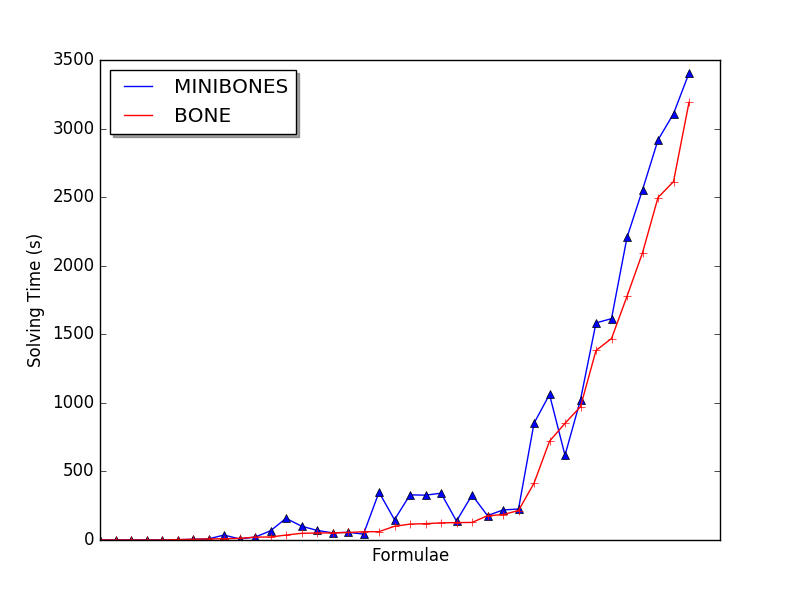
\includegraphics[scale=0.5]{ind.png}
   \caption{Solving Time Comparison on Industrial Formulae}
   \label{fig:ind}
\end{figure}

Figure \ref{fig:cs}(b) is the adjacent structure of formulae that can't be solved in 16000 seconds using both tools. It's obvious that there is no clear partition among the variables.


\begin{figure}[t]
\centering
\subfloat[Formulae with clear variables partition]{

\centering
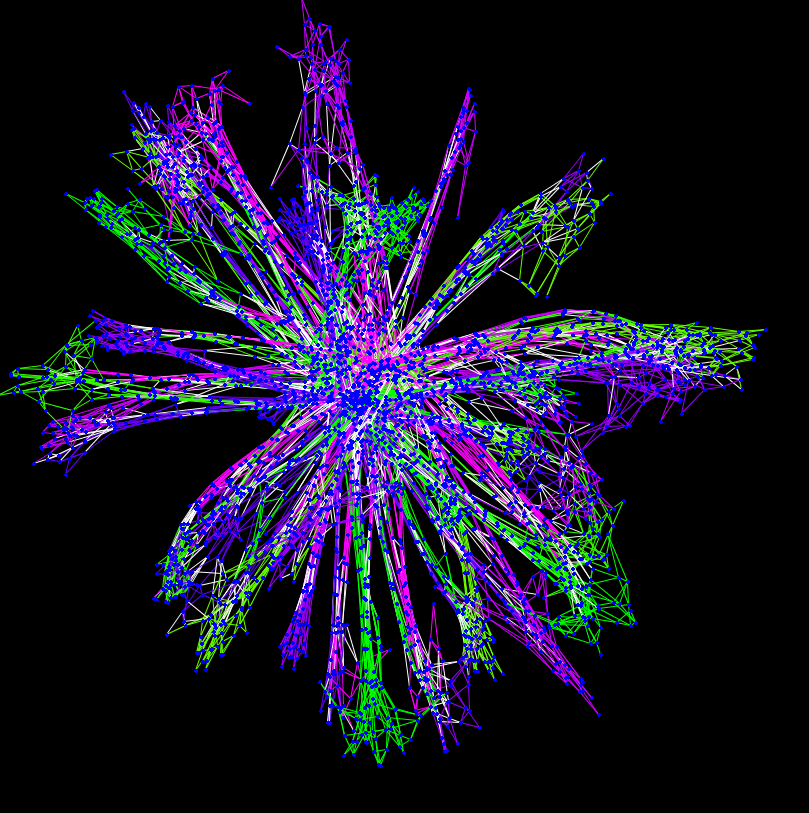
\includegraphics[width=.5\linewidth-0.45mm]{star.png}
}
\subfloat[Formulae with a tightly co-related variables]{
\centering
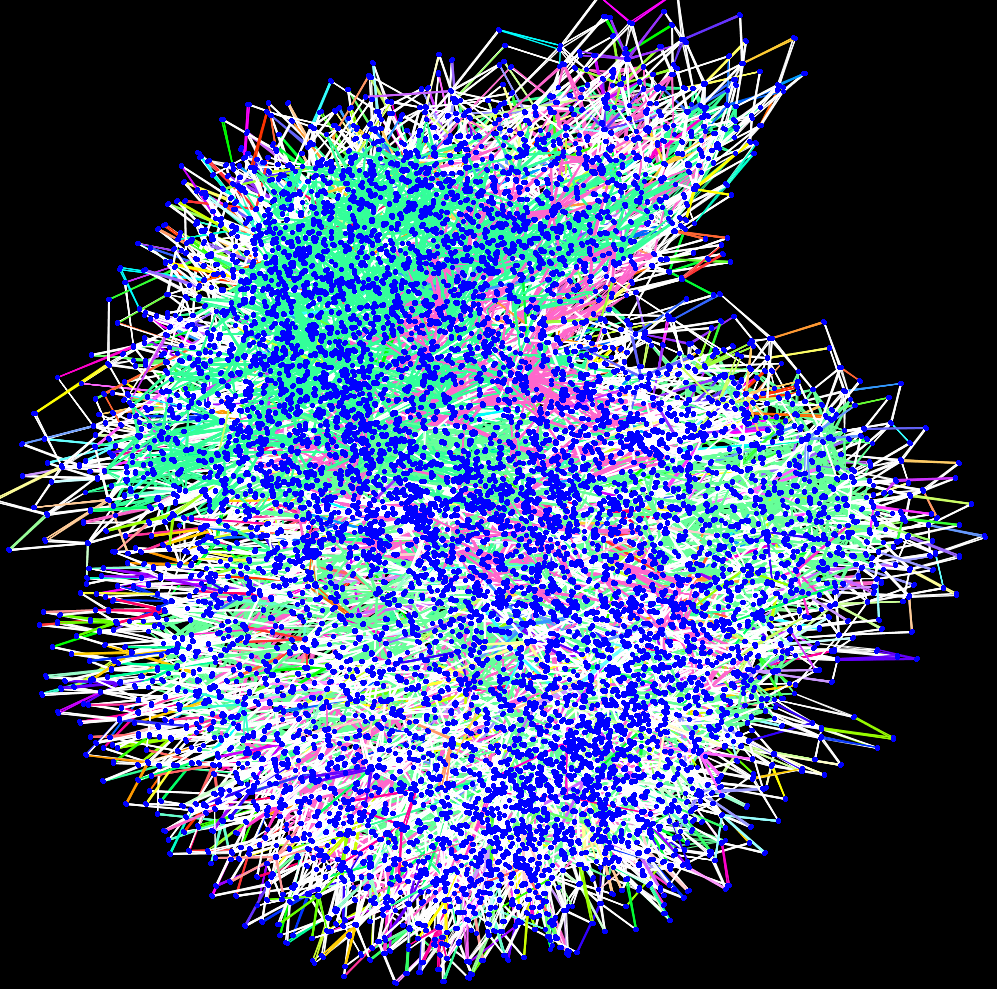
\includegraphics[width=.5\linewidth-0.45mm]{ball.png}
}
\caption{Adjacent structures}
\begin{minipage}[t]{0.9\textwidth} \small
\textit{(Figure (a) shows the star-like adjacent structure, indicates that variables separate into individual partitions, both \tool and \minibones are able to solve these formulae in 3600 seconds, \tool saved 34\% solving time in total. \\
Figure (b) shows the adjacent structure with a core and no branches, indicates that variables are tightly co-related in the formula. These formulae are more complex than the formula in \ref{fig:cs}(a), \tool solved 2 more formulae than \minibones among these formulae, within 16000 seconds)}
\end{minipage}

\label{fig:cs}
\end{figure}

For industrial formulae, \tool performs better than \minibones in general. We also found that the performance of \tool and \minibones are related to the adjacent structure of the given formula. A formula with clear partitions of variables tend to performs better on both \tool and \minibones.
To analysis the relations between formula structure and the performance of both tools, we designed and implemented experiments with 86 groups of generated formulae, consists of 6600 formulae in total. Every formula shares the same structure feature with other formula in the same group. All formulae shared the same number of variables and clauses.

\subsection{Results for Random Formulae}
Among all the 6600 random formulae, both \tool and \minibones are able to solve them within 50 seconds. Table \ref{tab:mcs_all} shows the total solving time and total SAT testings number of \tool and \minibones. 0.4\% solving time and 0.1\% SAT testings are saved by \tool.

\begin{table}[t]
\centering
\begin{tabular}{ccc}
\toprule
  &$\textbf{Solving Time}$ & $\textbf{SAT Testings Number}$ \\
\midrule
\tool & 50184 & 1508723  \\
\minibones & 50414 & 1532372 \\

\bottomrule
\end{tabular}
\caption{Solving Time and SAT Tests Number Comparison on Random Formulae}
\label{tab:mcs_all}
\end{table}

We separate the formulae into 86 groups according to the original unsatisfiable formula. \tool needs less solving time among 58 of them. Inherited from the industrial experiment, we consider the adjacent structures of different groups. Among all the 6600 generated formulae, \tool performs better for most of the case if there are more than 210 variables that have more than 10 adjacent variables. We refer variables with more than 10 adjacent variables as $\textit{active variables}$ since they appears in many clauses. It's obvious that with more active variables, the formula is more complex. We randomly select 10 formulae groups and demonstrate the average active variables number and total solving time of both tools in Table \ref{tab:mcs}. We can observe that most of the formulae performs better on \tool have more than 210 active variables.

\begin{table}[t]
\centering
\begin{tabular}{ccccc}
\toprule
Active Variables Number & $\textbf{st}$ of \tool(s) & $\textbf{st}$ of \minibones(s) & $\textbf{st}$ Difference\\
\midrule
203 & 354 & 346 & -2\% \\
208 & 614 & 574 & -6\% \\
215 & 346 & 400 & \textbf{13\%} \\
211 & 854 & 903 & \textbf{5\%} \\
215 & 365 & 381 & \textbf{4\%} \\
201 & 475 & 469 & -2\% \\
216 & 626 & 669 & \textbf{6\%} \\
204 & 643 & 592 & -7\% \\
208 & 389 & 424 & \textbf{8\%} \\
214 & 580 & 616 & \textbf{6\%} \\

\bottomrule
\end{tabular}
\caption{Active Variables Number and Solving Time of 10 Selected Random Formuale}
\label{tab:mcs}
\end{table}




%\section{Related Work}\label{sec:relw}
% This paper is concerned with computing backbones of propositional formulae, which was oriented from coloring problem \cite{CJG2001}, with a wide range of practical applications such as MaxSAT \cite{MMBM2005}.

%A number of backbones extraction algorithms have been proposed in recent years.
Kaiser and K\"{u}hlin proposed three model enumeration based algorithms for computing backbones \cite{KKW2001} using SAT solvers.
%The first one iteratively assigns true (false) to each variable and tests the resulting formula for satisfiability.
%The second one reuse the results of previous satisfiability checks and the last one maximizes the number of variables that
%an be classified without satisfiability checking, which share same purpose as our work.
%
Dubois and Dequen proposed a heuristic search for computing backbones of hard 3-SAT formulae which yields DPL-type algorithms with a significant
performance improvement over the best previous algorithms \cite{DD2001}.
Climer et al. proposed a graph-based approach to discover backbones which approximates lower and upper bounds to compute
backbones \cite{CZ2002}.% of instances of the travelling salesman problem .
%Kilby et al. showed that backbones are hard even to approximate and proposed algorithms for computing backdoors which little overlap with backbones \cite{KPS2005}.
%and proposed algorithms for computing backdoors, that are literals/variables whose absence will simplify formulas to be solved in polynomial time %\cite{KPS2005}. As discussed by \cite{KPS2005}, backbones have little overlap with backdoors.
%
%
Zhu et al, proposed an iterative SAT testing based algorithm \cite{ZWSM11,ZWM11} which is more efficient than previous model enumeration.
%At the first step, this algorithm assigned the first model returned from SAT solver to backbone estimation, which need less memory to compute backbone.

Marques-Silva et al.  investigated algorithms for computing backbones emphasizing the integration of existing algorithms which include model enumeration, iterative SAT-testing and filtering with modern SAT solvers, as well as optimisations.
They conducted an experimental evaluation of existing techniques and showed that backbone computation for large practical formulae is feasible. \cite{MJML2010,JLMS12,JLM15}.
%In this work, we proposed a novel Greedy-Whitening based approach \tool.
%Experimental results demonstrated that our approach performs better than the best one of algorithms in \cite{MJML2010,JLMS12,JLM15} for industrial formulae and
%hard random formulae, while for simple formulae, \tool is also comparable.





%The algorithm maintained an estimation of backbone. In each iteration, a clause that formed by the negation of backbone estimation is added to $\Phi$. If $\Phi$ was satisfiable, it implied that at least one non-backbone literal is in the backbone estimation. Intersection between the model given by SAT solver and the backbone estimation indicates the non-backbone literal. In this way, non-backbone literal is removed, the process is repeated until $\Phi'$ is not satisfiable any longer. Along with the estimation, the clauses number of $\Phi$  is monotone increasing due to the continuously insertion in each iteration, which dramatically promote the complexity of $\Phi$. In other words, for each iteration, it takes longer CPU time than the last iteration.

%Janota et al, proposed an Iterative algorithm (one test per variable) \cite{JLM15}. For each iteration, it added only one unit clause to the original formula, which made the new formula easier. Inspired by this algorithm, our approach in this paper follows this idea.

%The Core Based Algorithm presented in \cite{JLM15} is stable and effectiveness. The cb100 tool, as our main comparative object, was based on this algorithm. %Instead of adding only one unit clause to the original formula, this algorithm added all the unit clause to the formula. It will dramatically accelerate SAT solving. Although there is a high possibility that the new formula is unsatisfiable, whenever there was only one literal in unsatisfiable reason of the new formula, this literal is a backbone literal. In this way, it was able to find backbone literals with little cost. In this paper, the author showed that for formulae with backbone percentages lower than 25\%, Core Based Algorithms are better.
%significantly better. When the percentage of backbone is over 25\%, Core Based Algorithm behave very similarly Iterative SAT Testing Algorithm.


%Kilby et al proposed \cite{KST2005} that there was little overlap between backbone and backdoors.

%In \cite{KKW2001}, they partitioned backbone into inadmissible and necessary group. For inadmissible group, literals were false in each satisfying variable assignment. For necessary group, literals were true in each satisfying variable assignment. They described and compared three algorithms for searching the set of necessary and inadmissible variables, a basic iterative testing and two enhancements. The first enhancement was reusing the result of satisfiability checks to get more models for free, the second enhancement was selecting the decision variables for SAT solvers according to the previous information of inadmissible and necessary group.


%In \cite{DOG2001}, they proposed a heuristic search for backbone, and choose this backbone variables as branch nodes for the tree developed by a DPL-type procedure. Experiments showed that a significant performance improvement over the best current algorithms, and enhanced the scalability of the algorithm up to 700 variables.

%In \cite{WS2001}, they concluded the correlation of backbone size with the problem of optimization and approximation, using graph coloring, Travel Salesman, Number partition and block words planning. And they suggested that it is necessary to eliminate trivial cases of backbone before using backbone size to evaluate the hardness of optimization and approximation problems.


\section{Conclusions}\label{sec:conc}
%This paper proposes a novel greedy-whitening based approach(\tool, for short) to compute backbone of a propositional formulae.
%\tool first computes an under-approximation of non-backbone, which can save SAT solving counts and running time of the formula.
%Then, based on the under-approximation of non-backbone, \tool computes the over-approximation of backbone, which helps \tool to find a backbone literal %earlier.
%Finally, \tool iteratively tests literals to see if they are backbone literals, which is inspired by Iterative Algorithm.

%The experimental results show our approach is efficient, especially for industrial formulae which need longer time to compute the first model.
%Future improvements to backbone computation algorithms include parallel approximations, automatically identification of partitions and more accurate community %structure analysis.


%\section{Conclusion}\label{sec:conc}
In this paper, we proposed a backbone computing approach named \tool, using Greedy-Whitening based algorithm.
First, we computed an under-approximation of non-backbone $\NBLap(\Phi)$ using Greedy-based Algorithm in $O(n^2)$ time. Literals in $\NBLap(\Phi)$ didn't need an iterative SAT testing which can save of solving time.
%the saving of SAT testings resulted in the saving of solving time.
Next, we computed an approximation of backbone $\BLap(\Phi)$ using Whitening-based Algorithm. The elements in $\BLap(\Phi)$  would be backbone with high possibility. We iteratively extended the set of clauses $W_c$ and variables $W_v$ accordingly. $\BLap(\Phi)$ was the complement of $W_v$. Experiments showed that the proportions of backbone in $\BLap(\Phi)$ were higher than that in the original formula. Finding more backbone earlier will expedite backbone computing. It's because that more known backbone can prune more states in SAT solving.
At last, we iteratively confirmed backbone from previous approximations.

We compared \tool with state-of-art tool \minibones, on both industrial formulae and random formulae.
Experimental results for industrial formulae demonstrated that both \tool and \minibones were able to solve 34 formulae from 72 formulae in 3600 seconds. Among the three industrial groups, \tool saved 21\% solving time in total than \minibones does. \tool performed the best in $\textit{manthey}$ group. For every formula in $\textit{manthey}$, \tool needed less solving time than \minibones does.
\tool solved 49 formulae while \minibones solved 47 formula when the time limit was 16000 seconds.
On the other hand, \tool saved 0.4\% solving time compared to \minibones among 6600 random formulae.
Experiments on 6600 formulae indicated that \tool outperforms \minibones if more than 84\% variables have over 10 adjacent variables.

Industrial formulae have more complex adjacent structures than random formulae, since the scale of industrial formulae are larger. \tool performs better on industrial formulae than random formulae.

There were two major strategies used in Greedy-Whitening Algorithm, experiments showed that they performed differently on different benchmarks when applied independently, it opens a possibility for portfolio approach. How to decide which strategy to use on a given benchmark is the most important part portfolio approach.



%\input {algorithm_unique_satisfy.tex}


\newpage
\bibliography{bib}
\bibliographystyle{jair}

\end{document}
